\section{Possesso}

In Rust ogni valore introdotto nel programma è \textbf{posseduto} da una ed una sola variabile e il suo valore salvato in memoria.
\begin{itemize}
  \item Il \textbf{Borrow Checker} verifica formalmente questo fatto per ogni punto dell'esecuzione del programma
  \item Ogni violazione porta ad un \textbf{fallimento} della compilazione del programma con conseguente errore e spiegazione di quest'ultimo.
\end{itemize}

Possedere un valore significa essere responsabile del suo \textbf{rilascio}.

In particolare se il valore contiene una risorsa quale un puntatore a memoria dinamica, handle di file o socket, etc, questa deve essere liberata. Una volta liberata deve essere restituita al proprietario cui molto spesso è il Sistema Operativo.

Il rilascio avviene quando la variabile che possiede  esce dal proprio scope sintattico o quando viene \textbf{assegnata} ad un nuovo valore.

Rust offre un meccanismo di drop mediante il quale è possibile associare azioni arbitrarie da eseguire prima che sia liberata la memoria.
Il rilascio può essere rimandato ad un secondo momento se il contenuto della variabile viene trasferito (mosso) in un'altra variabile, la quale diventa responsabile del suo rilascio.\newline



\noindent
\begin{tcolorbox}
  \textbf{Nota:} Questo meccanismo rende l'utilizzo del Garbage collector, presente in linguaggi di programmazione come Java o Python, non necessario.
\end{tcolorbox}



\begin{center}
  \begin{minipage}{0.85\linewidth}
    % Primo blocco: 50% dello spazio per il codice
    \begin{minipage}{0.6\linewidth}
      \begin{minted}[breaklines]{rust}
fn main() {
    let mut v = Vec::with_capacity(4);  
    // v possiede il vec
    
    for i in 1..=5 {
        v.push(i);
    }
    
    println!("{:?}",v);
}        
\end{minted}
    \end{minipage}% <-- IMPORTANTE: il simbolo % qui evita spazi bianchi extra
    \hfill % Spazio elastico automatico per distanziare i due blocchi
    % Secondo blocco: 40% dello spazio per l'immagine
    \begin{minipage}{0.40\linewidth}
      \centering
      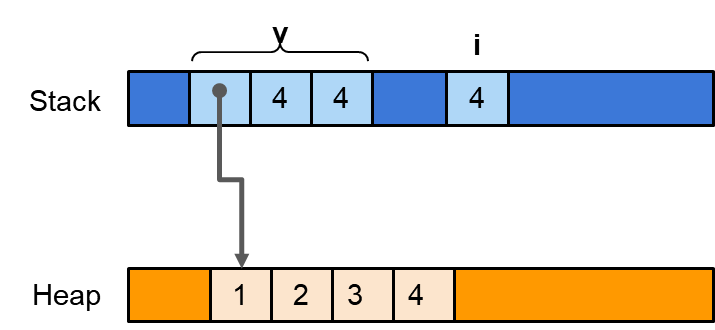
\includegraphics[width=\linewidth]{images/API_Programming/Possesso/Possesso-esempio1.png}
    \end{minipage}
  \end{minipage}
\end{center}

Inserendo valori all'interno del vettore, lo spazio
precedentemente allocato viene via via riempito. Se necessario il blocco viene riallocato per fare spazio ad un maggior numero di elementi.\newline

Finché le variabili sono in scope, \textit{i} e \textit{v}, le risorse che posseggono sono accessibili. Una volta usciti dal proprio scope la variabile si occupa dello smaltimento della porzione di stack, ed eventualmente heap, precedentemente allocato seguendo le informazioni contenute in Drop.


\section{Movimento}

Quando una variabile viene inizializzata, essa prende il possesso del relativo valore. Se ad una variabile mutable viene assegnato un nuovo valore, quello precedentemente posseduto viene rilasciato e la variabile diventa proprietaria del nuovo valore.

\begin{center}
  \mintinline{rust}{let mut b = a} \qquad\qquad \mintinline{rust}{f(a)} \qquad\qquad \mintinline{rust}{return a}
\end{center}

In questi tre casi, assegnazione, passaggio ad una funzione e ritorno di una variabile, in Rust, succede qualcosa che in altri linguaggi di programmazione non succede: il valore viene \textbf{mosso}, il possesso viene passato dalla variabile originale alla destinazione.

Questo porta ad alcune particolarità:

\begin{itemize}
  \item La variabile originale cessa di possedere il valore, ovvero non è più responsabile della sua distruzione ed il possesso passa alla variabile di destinazione, o parametro della funzione invocata
  \item La variabile originale rimane allocata fino a quando non termina la sua visibilità, ovvero al chiusura del blocco in cui è stata definita
  \item Accessi in \textbf{lettura} porteranno ad \textbf{errori di compilazione}
  \item Accessi in \textbf{scrittura} alla variabile originale avranno successo e ne riabiliteranno la lettura (si crea un nuovo oggetto)
  \item La variabile destinazione conterrà una copia bit a bit del valore originale, ammesso che il compilatore non riesca a riusare i dati originali al loro posto
\end{itemize}


\begin{center}
  \begin{minipage}{0.85\linewidth}
    % Primo blocco: 50% dello spazio per il codice
    \begin{minipage}{0.6\linewidth}
      \begin{minted}[breaklines]{rust}
let mut s1 = “hello”.to_string();
println!(“s1: {}”, s1);

let s2 = s1;
println!(“s2: {}”, s2);

//s1 non è più accessibile     
...
s1 = “world”.to_string();   \\s1 ritorna accessibile
\end{minted}
    \end{minipage}% <-- IMPORTANTE: il simbolo % qui evita spazi bianchi extra
    \hfill % Spazio elastico automatico per distanziare i due blocchi
    % Secondo blocco: 40% dello spazio per l'immagine
    \begin{minipage}{0.40\linewidth}
      \centering
      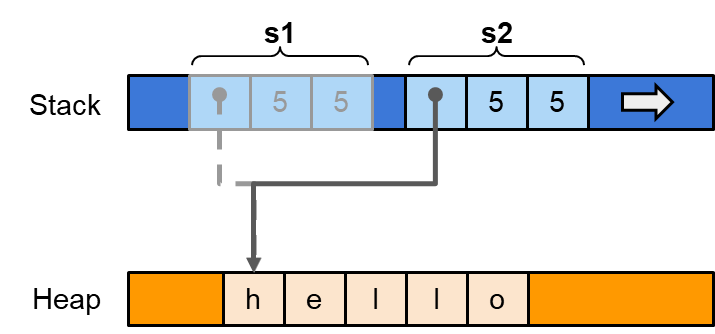
\includegraphics[width=1\linewidth]{images/API_Programming/Possesso/Possesso-esempio2.png}
    \end{minipage}
  \end{minipage}
\end{center}

Il movimento in Rust è la soluzione al problema del doppio possesso di parti di aree di memoria. Fisicamente nessuno ha cancellato l'area di memoria ma il compilatore marca $s1$ come inaccessibile.\newline




Il movimento previene l'ambiguità che introduce C/C++: un puntatore è valido/non valido, dobbiamo rilasciare noi la memoria o ci pensa qualcun altro?
In Rust è solo il possessore, univoco,  della variabile ad occuparsene, i precedenti possessori altro non fanno che contrarre lo stack per liberare lo spazio occupato.


\begin{minted}[breaklines]{rust}
let mut s1 = “hello”.to_string();
let mut s2 = s1 \\s2 possiede "hello"
...
let mut s1 ...  \\Questo s1 nasconde il precedente s1
\end{minted}

\newpage
\section{Copia}
Alcuni tipo, tra cui quelli numerici, sono definiti \textbf{copiabili}.

Questa proprietà è definita attraverso il tratto \textbf{Copy}.
Quando una valore assegnato ad un'altra variabile o usato come argomento in una chiamata a funzione, il valore originale rimane accessibile in \textbf{sola lettura}.

Questo è possibile quando il valore contenuto non costituisce una risorsa che richiede altre azioni di rilascio come ad esempio possono essere File o Socket.\newline

Se $Vec$ e $String$ posseggono il tratto \textit{Drop}, etichetta per lo smaltimento specifico dato che sono puntatori a zone di heap, $Int$, $Bool$, etc. assumono il tratto \textit{Copy}.\newline

\noindent
\begin{tcolorbox}
  \textbf{Nota:} Drop e Copy sono mutualmente esclusivi. Posso esistere anche tipi né Copy né Drop come per esempio gli oggetti Thread.
\end{tcolorbox}

I tipo semplici e le loro combinazioni, tuple e array di numeri, sono copiabili. Sono copiabili anche i riferimenti a valori non mutabili.

Viceversa i riferimenti a valori mutabili NON sono copiabili.\newline

\begin{figure}
  \centering
  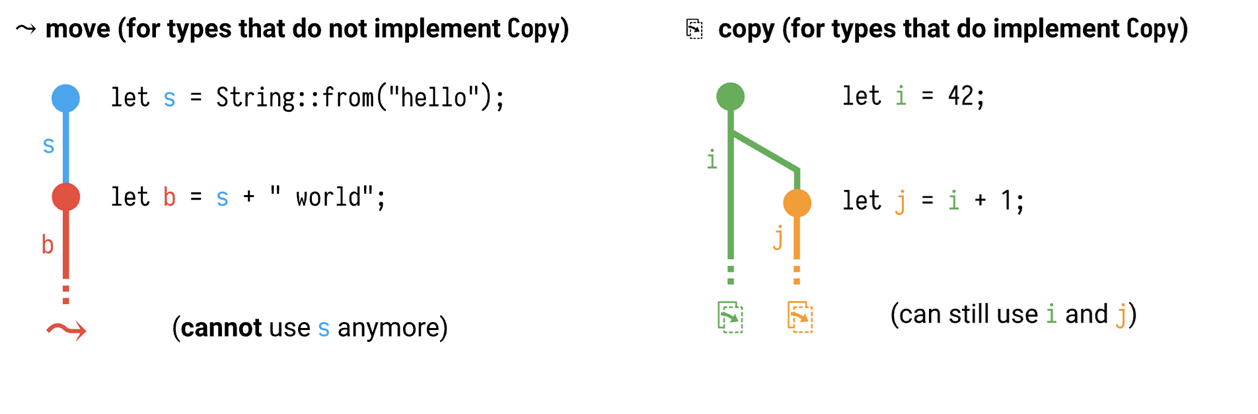
\includegraphics[width=0.85\linewidth]{images/API_Programming/Possesso/Possesso-esempio3.png}
\end{figure}

\begin{tcolorbox}
  \textbf{Nota:} Dal punto di vista del codice genero, non cambia nulla tra copia e movimento. L'istruzione di assegnazione o passaggio come argomento comporta la duplicazione, bit a bit, del valore originale. In caso di copia il Borrow Checker non impedisce l'ulteriore accesso in sola lettura al dato originale.
\end{tcolorbox}

\subsection{Copia e Movimento}

Copia e Movimento diventano esattamente la medesima istruzione assembly $mov$, quello che cambia sono le tabelle e le decisioni prese dal compilatore.


\begin{center}
  \begin{minipage}{0.85\linewidth}
    % Primo blocco: 50% dello spazio per il codice
    \begin{minipage}{0.6\linewidth}
      \begin{minted}[breaklines]{rust}
let string1 = "Hello".to_string();
let string2 = string1;  
//da qui in poi, string1 è inaccessibile in lettura
//a meno che non venga riassegnato
let num1: i32 = 3;
let num2 = num1; //nessun vincolo su num1!
\end{minted}
    \end{minipage}% <-- IMPORTANTE: il simbolo % qui evita spazi bianchi extra
    \hfill % Spazio elastico automatico per distanziare i due blocchi
    % Secondo blocco: 40% dello spazio per l'immagine
    \begin{minipage}{0.40\linewidth}
      \centering
      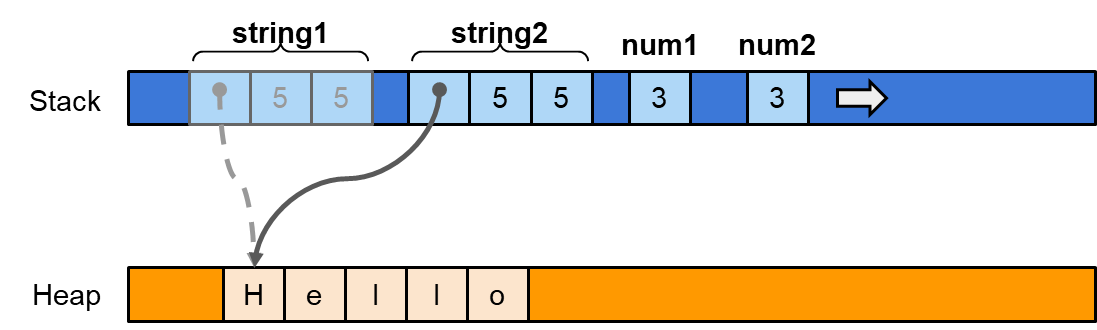
\includegraphics[width=1\linewidth]{images/API_Programming/Possesso/Possesso-esempio4.png}
    \end{minipage}
  \end{minipage}
\end{center}

\newpage
\section{Clonazione}

Alcune volte non vogliamo cedere il possesso ma solamente avere una copia e se un tipo implementa il tratto \textit{Clone} può essere duplicato invocando il metodo \textit{clone()}.

A differenza di copia e movimento, la clonazione può implementare una \textbf{copia profonda} dei valori. Questo implica un elevato costo di clonazione se il tipo risulta occupare molta memoria.\newline

L'implementazione dell'operazione di clonazione, a differenza di copia e movimento che sono sotto il controllo esclusivo del compilatore ed è basata sull'invocazione della funzione \textit{memcpy(...)}, è modificabile dal programmatore.\newline

\begin{tcolorbox}
  \textbf{Nota:} Affinché un tipo possa implementare il tratto Copy, occorre che implementi anche il tratto Clone. Tuttavia, non occorre che le due implementazioni coincidano.
\end{tcolorbox}


\begin{center}
  \begin{minipage}{0.85\linewidth}
    % Primo blocco: 50% dello spazio per il codice
    \begin{minipage}{0.6\linewidth}
      \begin{minted}[breaklines]{rust}
let mut s1 = "hi".to_string();
let s2 = s1.clone();

s1.push('!');

println!("s1: {}", s1); //hi!
println!("s2: {}", s2); //hi
\end{minted}
    \end{minipage}% <-- IMPORTANTE: il simbolo % qui evita spazi bianchi extra
    \hfill % Spazio elastico automatico per distanziare i due blocchi
    % Secondo blocco: 40% dello spazio per l'immagine
    \begin{minipage}{0.40\linewidth}
      \centering
      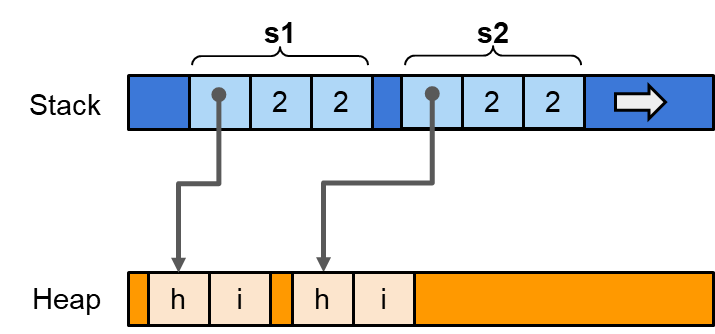
\includegraphics[width=0.8\linewidth]{images/API_Programming/Possesso/Possesso-esempio5.png}

      \vspace{0.1cm}

      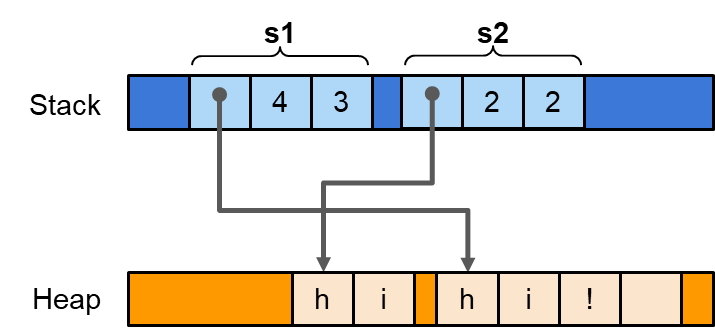
\includegraphics[width=0.8\linewidth]{images/API_Programming/Possesso/Possesso-esempio6.png}


    \end{minipage}
  \end{minipage}
\end{center}

\newpage
\section{Box<T> - Puntatore con possesso}

Una variabile locale è SEMPRE allocata sullo stack. Questo si estende di una quantità pari alla dimensione del valore che deve essere memorizzato nella variabile. Quando la variabile esce dal proprio scope sintattico, lo stack si contrae ed il valore viene rilasciato.

In alcune situazioni:

\begin{itemize}
  \item Non è nota la dimensione a priori
  \item Occorre prolungare il tempo di vita del valore oltre al blocco sintattico in cui è definito
  \item La dimensione è maggiore dello stack stesso
\end{itemize}

l'oggetto deve essere allocato sullo heap, utilizzando il tipo generico \textbf{Box<T>}. Una variabile di questo tipo contiene un puntatore al valore.

Per allocare un valore con il tipo Box si scrive:

\begin{center}
  \mintinline{rust}{let b = Box::new(v);}
\end{center}

dove \textit{v} è un qualsiasi valore. L'istruzione precedente definisce una variabile \textit{b} la quale è un puntatore ad un area di memoria sullo heap contenente il valore \textit{v}.

Si accede al valore contenuto con l'espressione \textit{*b}\footnote{Si può scrivere pure \textit{b.1}, il compilatore lo de-referenzia in autonomia (*b).1}, e se la variabile è definita come mutabile è possibile modificare il contenuto a cui si punta.\newline


\begin{center}
  \begin{minipage}{0.85\linewidth}
    % Primo blocco: 50% dello spazio per il codice
    \begin{minipage}{0.6\linewidth}
      \begin{minted}[breaklines]{rust}
fn useBox() {
    let i = 4;
    let mut b = Box::new( (5, 2) );
    (*b).1 = 7;
    println!("{:?}", *b); // (5,7)
}
\end{minted}
    \end{minipage}% <-- IMPORTANTE: il simbolo % qui evita spazi bianchi extra
    \hfill % Spazio elastico automatico per distanziare i due blocchi
    % Secondo blocco: 40% dello spazio per l'immagine
    \begin{minipage}{0.40\linewidth}
      \centering
      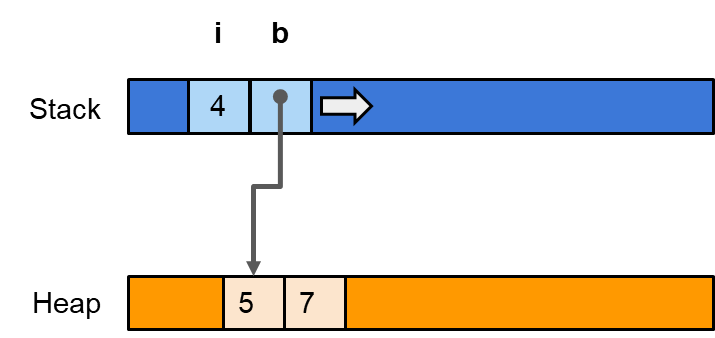
\includegraphics[width=1\linewidth]{images//API_Programming//Possesso/Possesso-esempio7.png}

    \end{minipage}
  \end{minipage}
\end{center}

Quando l'esecuzione del programma raggiungerà la fine del blocco di codice in cui la variabile \textit{b} è stata definita, il  blocco verrà rilasciata a patto che il contenuto di \textit{b}, il puntatore al blocco sia stato \textbf{mosso} in un'altra variabile.

\begin{center}
  \begin{minipage}{0.85\linewidth}
    % Primo blocco: 50% dello spazio per il codice
    \begin{minipage}{0.6\linewidth}
      \begin{minted}[breaklines]{rust}
fn makeBox(a: i32) -> Box<(i32,i32)> {
    let r = Box::new( (a, 1) );
    return r;
}


fn main() {
    let b = makeBox(5);
    let c = b.0 + b.1;
}
\end{minted}
    \end{minipage}% <-- IMPORTANTE: il simbolo % qui evita spazi bianchi extra
    \hfill % Spazio elastico automatico per distanziare i due blocchi
    % Secondo blocco: 40% dello spazio per l'immagine
    \begin{minipage}{0.40\linewidth}
      \centering
      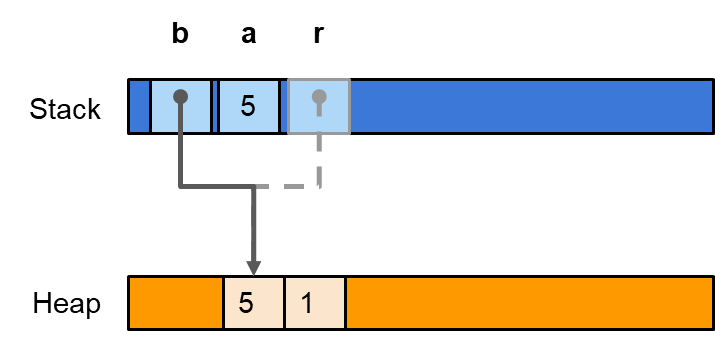
\includegraphics[width=1\linewidth]{images//API_Programming//Possesso/Possesso-esempio8.png}

      \vspace{0.1cm}

      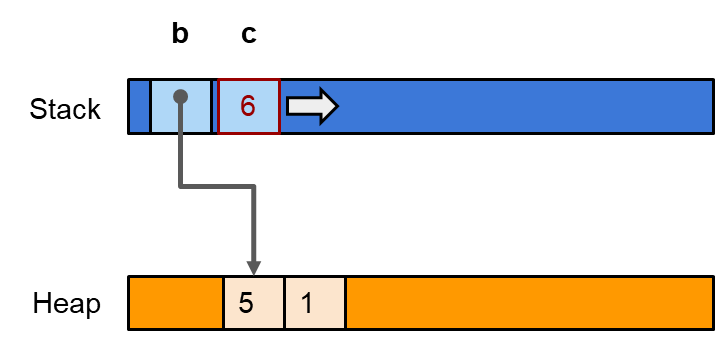
\includegraphics[width=1\linewidth]{images//API_Programming//Possesso/Possesso-esempio9.png}


    \end{minipage}
  \end{minipage}
\end{center}

\newpage
\section{Riferimenti}
Per risolvere i problemi di accesso, Rust introduce diverse forme di puntatori, volte a rendere espliciti responsabilità e diritti di chi le maneggia.
Il borrow checker si occupa di garantire che il codice sia scritto in conformità con tali regole e impedisce la compilazione in caso contrario.

Un \textbf{riferimento} è un puntatore in sola lettura ad un blocco di memoria \textbf{posseduto da un'altra variabile}.

\begin{itemize}
  \item Permette di accedere ad un valore senza trasferirne la proprietà
  \item Il riferimento può esistere solo mentre esiste la variabile che possiede il dato
  \item non serve utilizzare \textit{*}, quando si accede al valore tramite l'operatore \textit{.}
\end{itemize}

\begin{minted}[breaklines]{rust}
let point = (1.0, 0.0); //point possiede il valore
let reference = &point; //reference PUÒ accedere al valore in lettura
//finché esiste point
println!(“({}, {})”, reference.0, reference.1);
\end{minted}


\subsection{Riferimenti e prestiti}

Un riferimento prende in prestito, borrows, in sola lettura, l'indirizzo di memoria in cui esiste il valore.

Fino a che il riferimento è accessibile, non è possibile modificare il valore, né tramite il riferimento, il quale è in sola lettura, né tramite la variabile che possiede il valore.\newline

È possibile creare ulteriori riferimenti a partire dal dato originale o da altri riferimenti ad esso.

\begin{itemize}
  \item I riferimenti sono \textbf{copiabili}: viene duplicato il puntatore
  \item Il compilatore, attraverso il BC, garantisce che un riferimento punti sempre ad un dato valido
  \item Finché esiste almeno un riferimento, il dato originale \textbf{non potrà essere né modificato né distrutto}
\end{itemize}

\subsection{Riferimenti mut - mutual exclusion}
A partire da una variabile che possiede un valore è possibile estrarre \textbf{un solo riferimento mutabile} per volta. \mintinline{rust}{let r = &mut v;}.


Mentre esiste un riferimento mutabile

\begin{itemize}
  \item Non possono esistere riferimenti semplici, in sola lettura
  \item Non è possibile modificare né muovere la variabile che possiede il valore
\end{itemize}

È possibile creare un riferimento mutabile solo se la variabile che possiede il dato è a sua volta dichiarata come mutabile.

\begin{figure}[htbp]
  \centering
  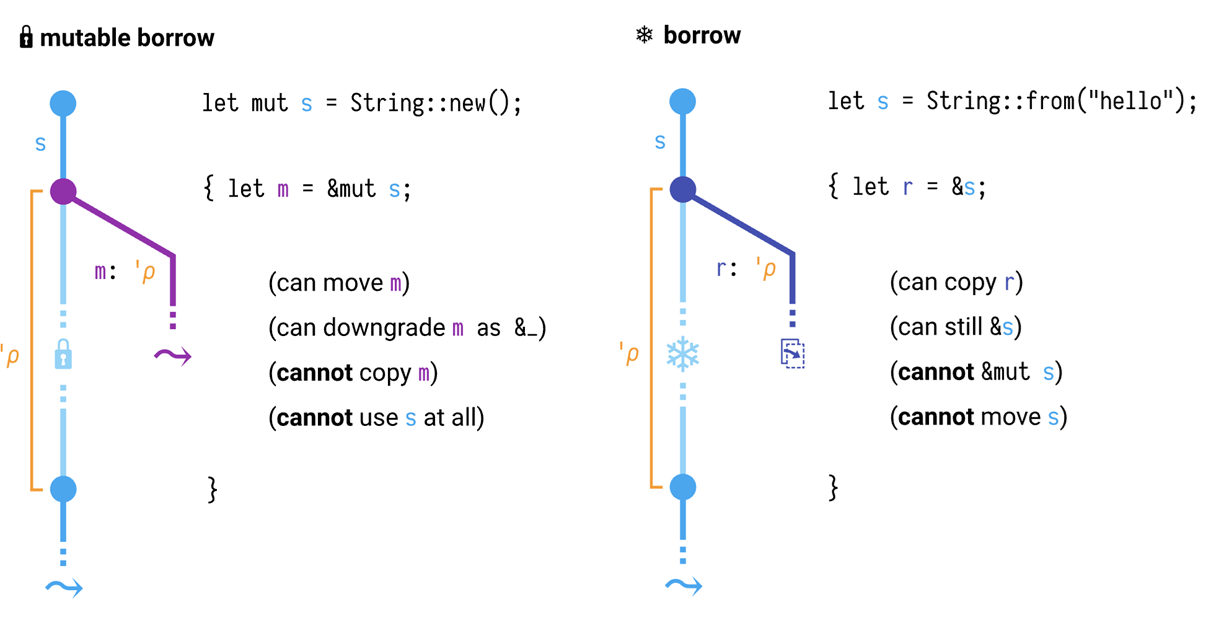
\includegraphics[width=0.55\linewidth]{images//API_Programming//Possesso/Possesso-esempio10.png}
\end{figure}

\newpage
\subsection{Riferimenti: disposizione in memoria}

I riferimenti sono implementati diversamente in base al tipo puntato

\begin{itemize}
  \item Puntatori semplici, se il compilatore conosce la dimensione del dato puntato
  \item Puntatore + dimensione (fat pointer), se la dimensione del dato è solo nota in fase di esecuzione. Nelle stringhe tolgo il problema di inserire il terminatore.
  \item Puntatore doppio, se il tipo di dato puntato è noto solo per l'insieme di tratti che implementa. Esempi File o Socket.
\end{itemize}


\begin{center}
  % --- ESEMPIO 1: SINGLE POINTER ---
  \begin{minipage}{0.85\linewidth}
    \begin{minipage}[c]{0.55\linewidth} % Colonna Codice (55%)
      \begin{minted}[breaklines]{rust}
let i: i32 = 10;
let r1: &i32 = &i;
            \end{minted}
    \end{minipage}
    \hfill
    \begin{minipage}[c]{0.30\linewidth} % Colonna Immagine (40%)
      \centering
      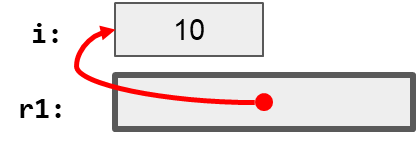
\includegraphics[width=\linewidth]{images/API_Programming/Possesso/Possesso-esempio13.png}
      \captionof{figure}{Single pointer}
    \end{minipage}
  \end{minipage}

  \vspace{0.3cm} % Spazio tra i vari esempi

  % --- ESEMPIO 2: FAT POINTER ---
  \begin{minipage}{0.85\linewidth}
    \begin{minipage}[c]{0.55\linewidth}
      \begin{minted}[breaklines]{rust}
let a: [i32;3] = [1,2,3];
let r2: &[i32] = &a;
            \end{minted}
    \end{minipage}
    \hfill
    \begin{minipage}[c]{0.40\linewidth}
      \centering
      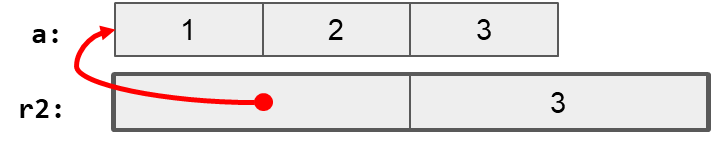
\includegraphics[width=\linewidth]{images/API_Programming/Possesso/Possesso-esempio14.png}
      \captionof{figure}{Fat pointer}
    \end{minipage}
  \end{minipage}

  \vspace{0.3cm}

  % --- ESEMPIO 3: DOUBLE POINTER ---
  \begin{minipage}{0.85\linewidth}
    \begin{minipage}[c]{0.55\linewidth}
      \begin{minted}[breaklines]{rust}
let f: File = File::create("test.txt");
let r3: &dyn Write = &f;
            \end{minted}
    \end{minipage}
    \hfill
    \begin{minipage}[c]{0.40\linewidth}
      \centering
      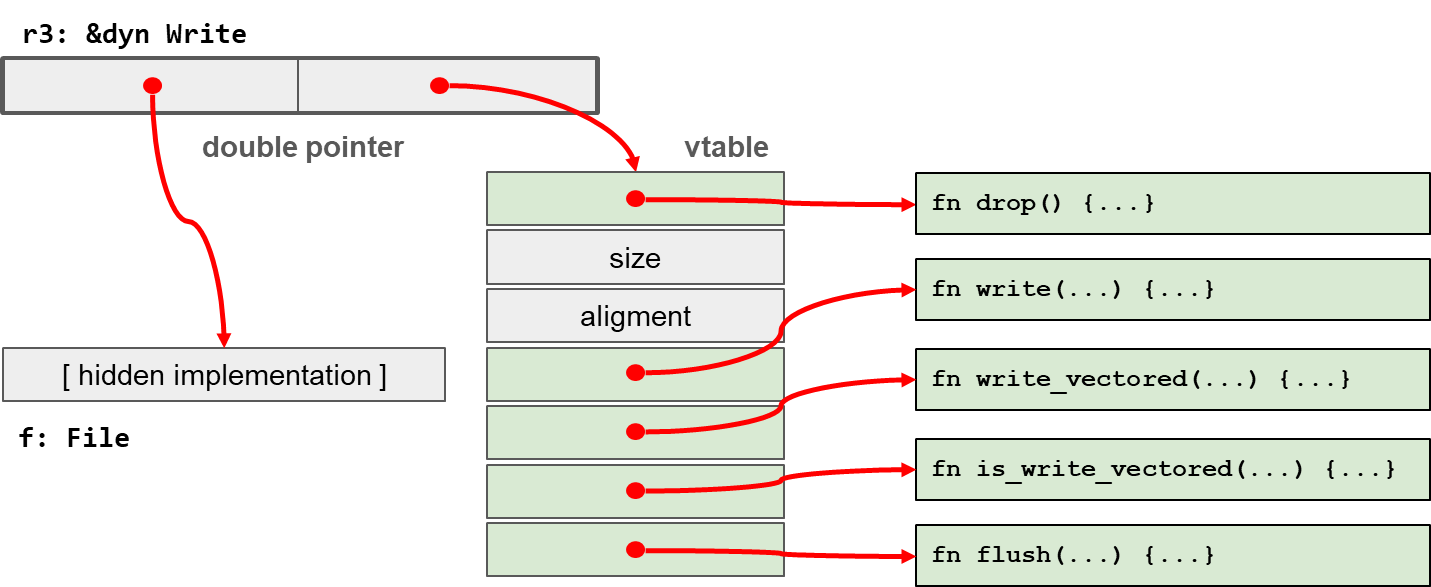
\includegraphics[width=\linewidth]{images/API_Programming/Possesso/Possesso-esempio15.png}
      \captionof{figure}{Double pointer}
    \end{minipage}
  \end{minipage}
\end{center}


\section{Tempo di vita dei riferimenti}
Il BC garantisce che tutti gli accessi ad un riferimento avvengano solo in un intervallo di tempo, o righe, compreso in quello in cui il dato esiste. Serve ad impedire il fenomeno dei \textbf{dangling pointer}.

L'insieme delle righe in cui si fa accesso al riferimento costituisce il suo \textbf{lifetime}. Tale info è mantenuta dal compilatore assieme ad altre informazioni, quale il tipo, e non ha alcuna rappresentazione in fase di esecuzione.\newline

Sebbene il tempo di vita in molte situazioni possa essere omesso, il tempo di vita di un riferimento può essere espresso nella firma del tipo. Questo aiuta sia il programmatore sia il compilatore per il mantenimento dell'informazione.

\begin{itemize}
  \item \mintinline{rust}{&'a NomeTipo}, dove \textit{a} è un identificativo qualsiasi e il simbolo ' serve a quantificarlo come tempo di vita
  \item Tale notazione è utile in quelle situazioni in cui occorre imporre vincoli sulla durata relativa dei tempo di vita di due o più riferimenti
\end{itemize}

Se un riferimento deve durare l'intera durata del programma viene indicato con \\\mintinline{rust}{&'static NomeTipo}.\newline

\begin{tcolorbox}
  \textbf{Nota:} Una stringa espressa in formato letterale ( "Some string") ha come tipo \mintinline{rust}{&'static str}, in quanto la sequenza di caratteri viene allocata dal compilatore nella sezione delle costanti e non viene mai rilasciata.
\end{tcolorbox}


Per essere lecito, il tempo di vita di un riferimento deve essere contenuto, minore, nel tempo di vita del valore a cui punta. Sempre il BC si fa carico di garantire il vincolo.\newline
Questo richiede di esplicitare il tempo di vita quando si memorizza un riferimento all'interno di una struttura dati, come per esempio una tupla, o si usa un riferimento come valore di ritorno di una funzione.\newline

Il vincolo (apparentemente ovvio) di esistenza in vita dei vincoli dovrebbe essere alla
base anche di tutti gli usi dei puntatori in C e C++.

Poiché, però, in questi linguaggi non viene tracciato il tempo di vita, il compilatore non è in grado di identificare la presenza di dangling pointers, né identificare eventuali problemi di non rilascio o doppio rilascio, come invece avviene in Rust.

\begin{minted}[breaklines]{rust}
{
    let r;
    {
        let x = 1;
        r = &x;
    }
    assert_eq!(*r, 1);
}

//error: `x` does not live long enough
\end{minted}


\subsection{Esistenza in vita}

Le regole, ovviamente, valgono anche quando si crea un riferimento ad una parte di una struttura dati più grande.

L'esistenza in vita del riferimento deve essere inclusa in quella della struttura a cui punta

\begin{minted}[breaklines]{rust}
let v = vec![1, 2, 3];
let r = &v[1]; // v deve durare più a lungo di r
\end{minted}

Se, al contrario si memorizzano dei riferimenti in una struttura, tutti questi riferimenti
devono avere una durata di vita maggiore della struttura dati in cui sono memorizzati.



\begin{minted}[breaklines]{rust}
{
    let mut v = Vec::new();
    {
        let a = 1;
        v.push(&a);
    }
    println!("{:?}", v);
}

\\error[E0597]: `a` does not live long enough
\end{minted}

\section{Riferimenti e funzioni}

Se una funzione riceve un parametro di tipo riferimento (mutabile o meno), il tempo
di vita del riferimento diventa parte integrante della firma della funzione
È necessario infatti che tutte le operazioni eseguite dalla funzione sul riferimento siano compatibili con la validità del dato memorizzato al suo interno

\begin{center}
  \mintinline{rust}{fn f(p: &i32) {...}} $\Rightarrow$ \mintinline{rust}{fn f<'a>(p: &'a i32) {...}}
\end{center}

Il compilatore provvede in molti casi a effettuare autonomamente la riscrittura indicata (lifetime
elision).\newline

Se la funzione riceve più riferimenti, può essere necessario indicare se il loro tempo
di vita sia vincolato al più breve o se siano disgiunti

\begin{itemize}
  \item Nel primo caso si usa un solo identificatore \mintinline{rust}{fn f<'a>(p1: &'a i32, p2:&'a i32) {...}}
  \item Nel secondo si usano etichette diverse \mintinline{rust}{fn f<'a, 'b>(p1: &'a i32, p2:&'b i32) {...}}
\end{itemize}

Uno dei casi più frequenti in cui il compilatore non riesce a dedurre il corretto
tempo di vita è legato a funzioni che restituiscono un riferimento, estratto da una
delle strutture dati ricevute in ingresso.

In tale caso occorre annotare il tipo restituito con la corretta etichetta

\begin{center}
  \mintinline{rust}{fn f<'a, 'b>(p1: &'a Foo, p2:&'b Bar) -> &'b i32 { /*...*/ return &p2.y; }}
\end{center}

Se la funzione memorizza il riferimento ricevuto in ingresso in una struttura dati, il
compilatore deduce che il tempo di vita della struttura in cui il riferimento è
memorizzato deve essere incluso o coincidente con il tempo di vita del riferimento.

Se questo non avviene, il compilatore identifica l'errore e impedisce alla compilazione di avere
successo.

\begin{minted}[breaklines]{rust}
fn f(s: &str, v: &mut Vec<&str>) {
    v.push(s);  //error: lifetime mismatch
}
\end{minted}

\begin{minted}[breaklines]{rust}
fn f<'a>(s: &'a str, v: &'a mut Vec<&str>) {
    v.push(s);
}
//error: explicit lifetime required in the type of `v`
\end{minted}

\begin{minted}[breaklines]{rust}
fn f<'a>(s: &'a str, v: &'a mut Vec<&'a str>) {
    v.push(s);
}

fn main() {
    let mut v: Vec<&str> = Vec::new();
    {
        let s= String::from("abc");
        v.push(&s);     //error: `s` does not live long enough
    }
    println!("{:?}",v);
}

\end{minted}

Se una funzione ha due o più riferimenti in ingresso e un riferimento in uscita, il
compilatore non è in grado di decidere (senza eseguire il codice) da quale
parametro provenga il riferimento in uscita. L'inserimento degli identificatori nella firma della funzione risolve questa ambiguità.

\begin{minted}[breaklines]{rust}
fn f<'b, 'c>(x: &'b S, y: &'c S) -> &'c u8 {...}

let v1 = S(1);
let mut v2 = S(2);

let r = f(&v1, &v2);    // Sappiamo che r è basato su v2,
                        // che rimane nello stato di prestito
                        // mentre v1 viene rilasciato e può evolvere
v2 = v1; // Questa operazione crea un problema!
print_byte(r); // Qui finisce il prestito di r (e di v2)
\end{minted}

Lo scopo degli identificatori relativi al ciclo di vita è duplice:

\begin{itemize}
  \item Per il codice che invoca la funzione (chiamante), essi indicano su quale, tra gli indirizzi in ingresso, è basato il risultato in uscita
  \item Per il codice all'interno della funzione (chiamato), essi garantiscono che vengano restituiti solo indirizzi cui è lecito accedere per (almeno) il tempo di vita indicato
\end{itemize}

All'atto dell'invocazione, gli identificatori forniti dal programmatore (o inseriti
automaticamente dal compilatore, quando possibile) sono legati all'effettivo
intervallo minimo (espresso come insieme di linee di codice) nel quale il valore da
cui il prestito è stato preso debba restare bloccato per non violare le assunzioni su
cui la funzione è basata.

Tentativi di modificare il valore originale da cui il prestito è preso prima che il tempo di vita sia trascorso portano ad errori di compilazione che costituiscono la base della robustezza del sistema di possesso e prestito offerto da Rust


\section{Riferimenti e strutture dati}

Lo stesso tipo di ragionamento vale se il dato viene salvato all'interno di una
qualsiasi struttura dati

\begin{itemize}
  \item Rust verifica che il valore a cui si punta abbia un tempo di vita maggiore o uguale del tempo di vita della struttura dati
  \item Questo richiede di esplicitare il tempo di vita della struttura rispetto al tempo di vita dei riferimenti in essa contenuti
\end{itemize}

Se una struttura che contiene riferimenti è contenuta, a sua volta, in un'altra
struttura, anche quest'ultima deve avere il tempo di vita specificato in modo
esplicito.

\begin{center}
  \begin{minipage}{1\linewidth}
    % Primo blocco: 50% dello spazio per il codice
    \begin{minipage}{0.50\linewidth}
      \begin{minted}[breaklines]{rust}
        struct User<'a> {
            id: u32,
            name: &'a str,
        }        
\end{minted}
    \end{minipage}% <-- IMPORTANTE: il simbolo % qui evita spazi bianchi extra
    \hfill % Spazio elastico automatico per distanziare i due blocchi
    % Secondo blocco: 40% dello spazio per l'immagine
    \begin{minipage}{0.50\linewidth}
      \begin{minted}[breaklines]{rust}
        struct Data<'a> {
            user: User<'a>,
            password: String,
        }     
\end{minted}
    \end{minipage}
  \end{minipage}
\end{center}


\section{Elisione dei tempi di vita}

Rust, per default, provvede ad assegnare, ad ogni riferimento presente in una struttura dati o tra i parametri di una funzione, un tempo di vita distinto. Tali tempi di vita si propagano al codice che fa uso di tale struttura dati e, in assenza di ambiguità, non richiede di esplicitare gli identificatori dei tempi di vita.

\begin{center}
  \centering
  \begin{minipage}{\linewidth}
    % Primo blocco: 50% dello spazio per il codice
    \begin{minipage}{0.50\linewidth}
      \begin{minted}[breaklines]{rust}
struct Point {
    x: &i32,
    y: &i32,
}

fun scale(r: &i32, p: Point) -> i32 {
    r * (p.x * p.x + p.y * p.y)
}       
\end{minted}
    \end{minipage}% <-- IMPORTANTE: il simbolo % qui evita spazi bianchi extra
    \hfill % Spazio elastico automatico per distanziare i due blocchi
    % Secondo blocco: 40% dello spazio per l'immagine
    \begin{minipage}{0.50\linewidth}
      \begin{minted}[breaklines]{rust}
struct Point {
    x: &'a i32,
    y: &'b i32,
}
fun scale<'a,'b,'c> (r: &'a i32, p: Point<'b, 'c>) -> i32 {
    r * (p.x * p.x + p.y * p.y)
}   
\end{minted}
    \end{minipage}
  \end{minipage}
\end{center}

Se una funzione restituisce un riferimento o un tipo che contiene - direttamente o
indirettamente - un riferimento, occorre disambiguare il tempo di vita del valore
ritornato

\begin{itemize}
  \item Se c'è un solo parametro in ingresso dotato di tempo di vita, Rust assume che quello debba essere il tempo di vita del risultato
  \item Se sono presenti più parametri in ingresso con tempo di vita, tocca al programmatore esplicitare quale debba essere il tempo di vita da associare al risultato
\end{itemize}

Nel caso di metodi che accedono a self tramite un riferimento, Rust assume che il
tempo di vita da associare al risultato sia quello del riferimento a self.

Questo parte dal presupposto che se un metodo di un oggetto restituisce un dato preso a prestito
(borrow), questo sia stato preso dai dati posseduti dall'oggetto stesso.


\section{Possesso - riassunto delle regole}

\begin{itemize}
  \item Ciascun valore ha un unico possessore (variabile o campo di una struttura). Il valore viene rilasciato (drop) quando il possessore esce dal proprio scope o quando al possessore
        viene assegnato un nuovo valore.
  \item Può esistere, al più, un singolo riferimento mutabile ad un dato valore

  \item \textbf{Oppure}, possono esistere molti riferimenti immutabili al medesimo valore. Ma fintanto che ne esiste almeno uno, il valore non può essere mutato.

  \item Tutti i riferimenti devono avere una durata di vita inferiore a quella del valore a cui
        fanno riferimento

\end{itemize}

\section{Puntatori in Rust}

\begin{table}[H]
  \renewcommand{\arraystretch}{1.6}
  \centering
  \begin{tabular}{>{\bfseries}l p{4.7cm} p{4.7cm}}
    % \hline
    \hline
    \textbf{Proprietà}     & \textbf{\&T}                                                                    & \textbf{Box<T>}                                 \\
    \hline
    Possesso               & No: prestito                                                                    & Possessore unico                                \\
    Rilascio               & A carico del possessore                                                         & Automatico al termine dello scope               \\
    Validità               & Garantita dal compilatore                                                       & Garantita in fase di esecuzione                 \\
    Nullabilità            & Mai nullo                                                                       & Mai nullo                                       \\
    Aliasing  e mutabilità & Controllata: o molti riferimenti in sola lettura o un solo riferimento mutabile & Soggetta alla regole del possesso (no aliasing) \\

    \hline
  \end{tabular}
\end{table}

\section{Slice}
Una slice (fetta) è una VISTA di una sequenza contigua di elementi, la cui lunghezza NON è nota in fase di compilazione, ma disponibile durante l'esecuzione.

Internamente viene rappresentata come una tupla di due elementi, il primo dei quali punta al primo valore della sequenza, mentre il secondo indica il numero di elementi consecutivi. Una slice di elementi T ha tipo [T].

Una slice \textbf{non possiede} i dati cui fa riferimento. Questi appartengono sempre ad un'altra variabile, da cui la slice viene derivata. Tutti i valori contenuti sono garantiti essere inizializzati, gli accessi sono verificati in fase di esecuzione.

È possibile ricavare una slice a partire da un array, ma anche da altri tipi di contenitori quali std::Vec<T>, String, Box<[T]>, etc.

\begin{minted}[breaklines]{rust}
let a: [i32; 5] = [1, 2, 3, 4, 5]; // a è un array di 5 interi
let s = &a[1..3]; // s è una slice formata da 2 elementi [2,3]
let two = s[0]; // two contiene il valore 2
\end{minted}

\begin{figure}[htbp]
  \centering
  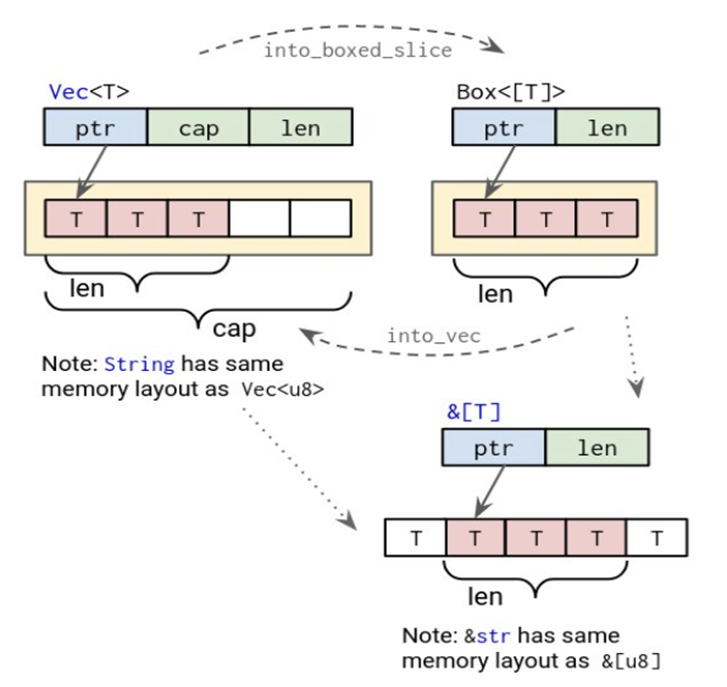
\includegraphics[width=0.4\linewidth]{images/API_Programming/Possesso/Possesso-slice.png}
\end{figure}

\newpage
\section{Vantaggi introdotti dal concetto di possesso}

Un programma Rust, pur non avendo un garbage collector, offre molteplici garanzie
relative alla correttezza degli accessi in memoria e del rilascio delle risorse.

\begin{itemize}
  \item Non esiste il concetto di \textbf{riferimento nullo} e, di conseguenza, non c'è il rischio di dereferenziarlo
  \item Poiché il borrow checker vigila sulle assegnazioni dei riferimenti e sugli intervalli temporali in cui essi sono effettivamente usati impedendo accessi illeciti, non c'è il rischio di originare errori di
        segmentazione o accesso illegale ad aree ristrette di memoria, né la possibilità di avere riferimenti ad aree già rilasciate (dangling pointer)
  \item Poiché in ogni istante il borrow checker è in grado di determinare la dimensione di un blocco di memoria cui un riferimento punta, non possono verificarsi \textbf{buffer overflow} né \textbf{buffer underflow}
  \item Per lo stesso motivo, gli iteratori offerti da Rust \textbf{non eccedono} mai i loro limiti
\end{itemize}

Tutte le variabili sono \textbf{immutabili} per default e occorre una dichiarazione esplicita
per renderle mutabili. Questo obbliga il programmatore a riflettere attentamente sul come e dove i dati debbano essere modificati e su quale sia il ciclo di vita di ciascun valore.

Il modello di possesso non riguarda solo la gestione della memoria, ma anche la
\textbf{gestione delle risorse} contenute in un valore come socket di rete, handle di file e database, descrittori dei dispositivi.

L'assenza di un garbage collector impedisce \textbf{comportamenti non deterministici}. In particolare, la sospensione totale del funzionamento ogni qual volta occorra ricompattare la
memoria.

\section{Disposizione in memoria}

\begin{figure}[htbp]
  \centering
  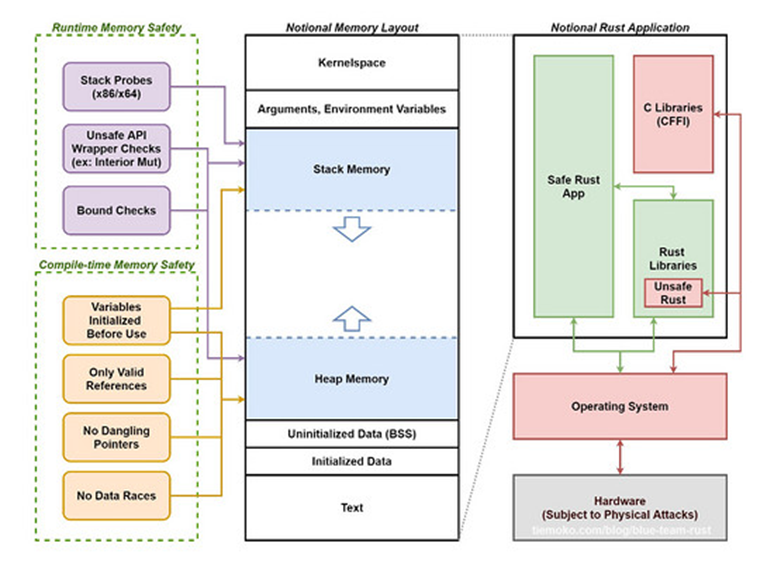
\includegraphics[width=0.6\linewidth]{images/API_Programming/Possesso/Possesso-disposizione-in-memoria.png}
\end{figure}
